\section{Example SMURF Program}

The SMURF program in Figure~\ref{fig:ex1} shows how to use various language features in SMURF including function definitions, keywords, types, library functions, and operators. The code uses the \texttt{trans} and \texttt{inver} library functions to generate two tone rows that are then used to create chords and a list of measures that make up a music score. 

\begin{figure}
        \centering
        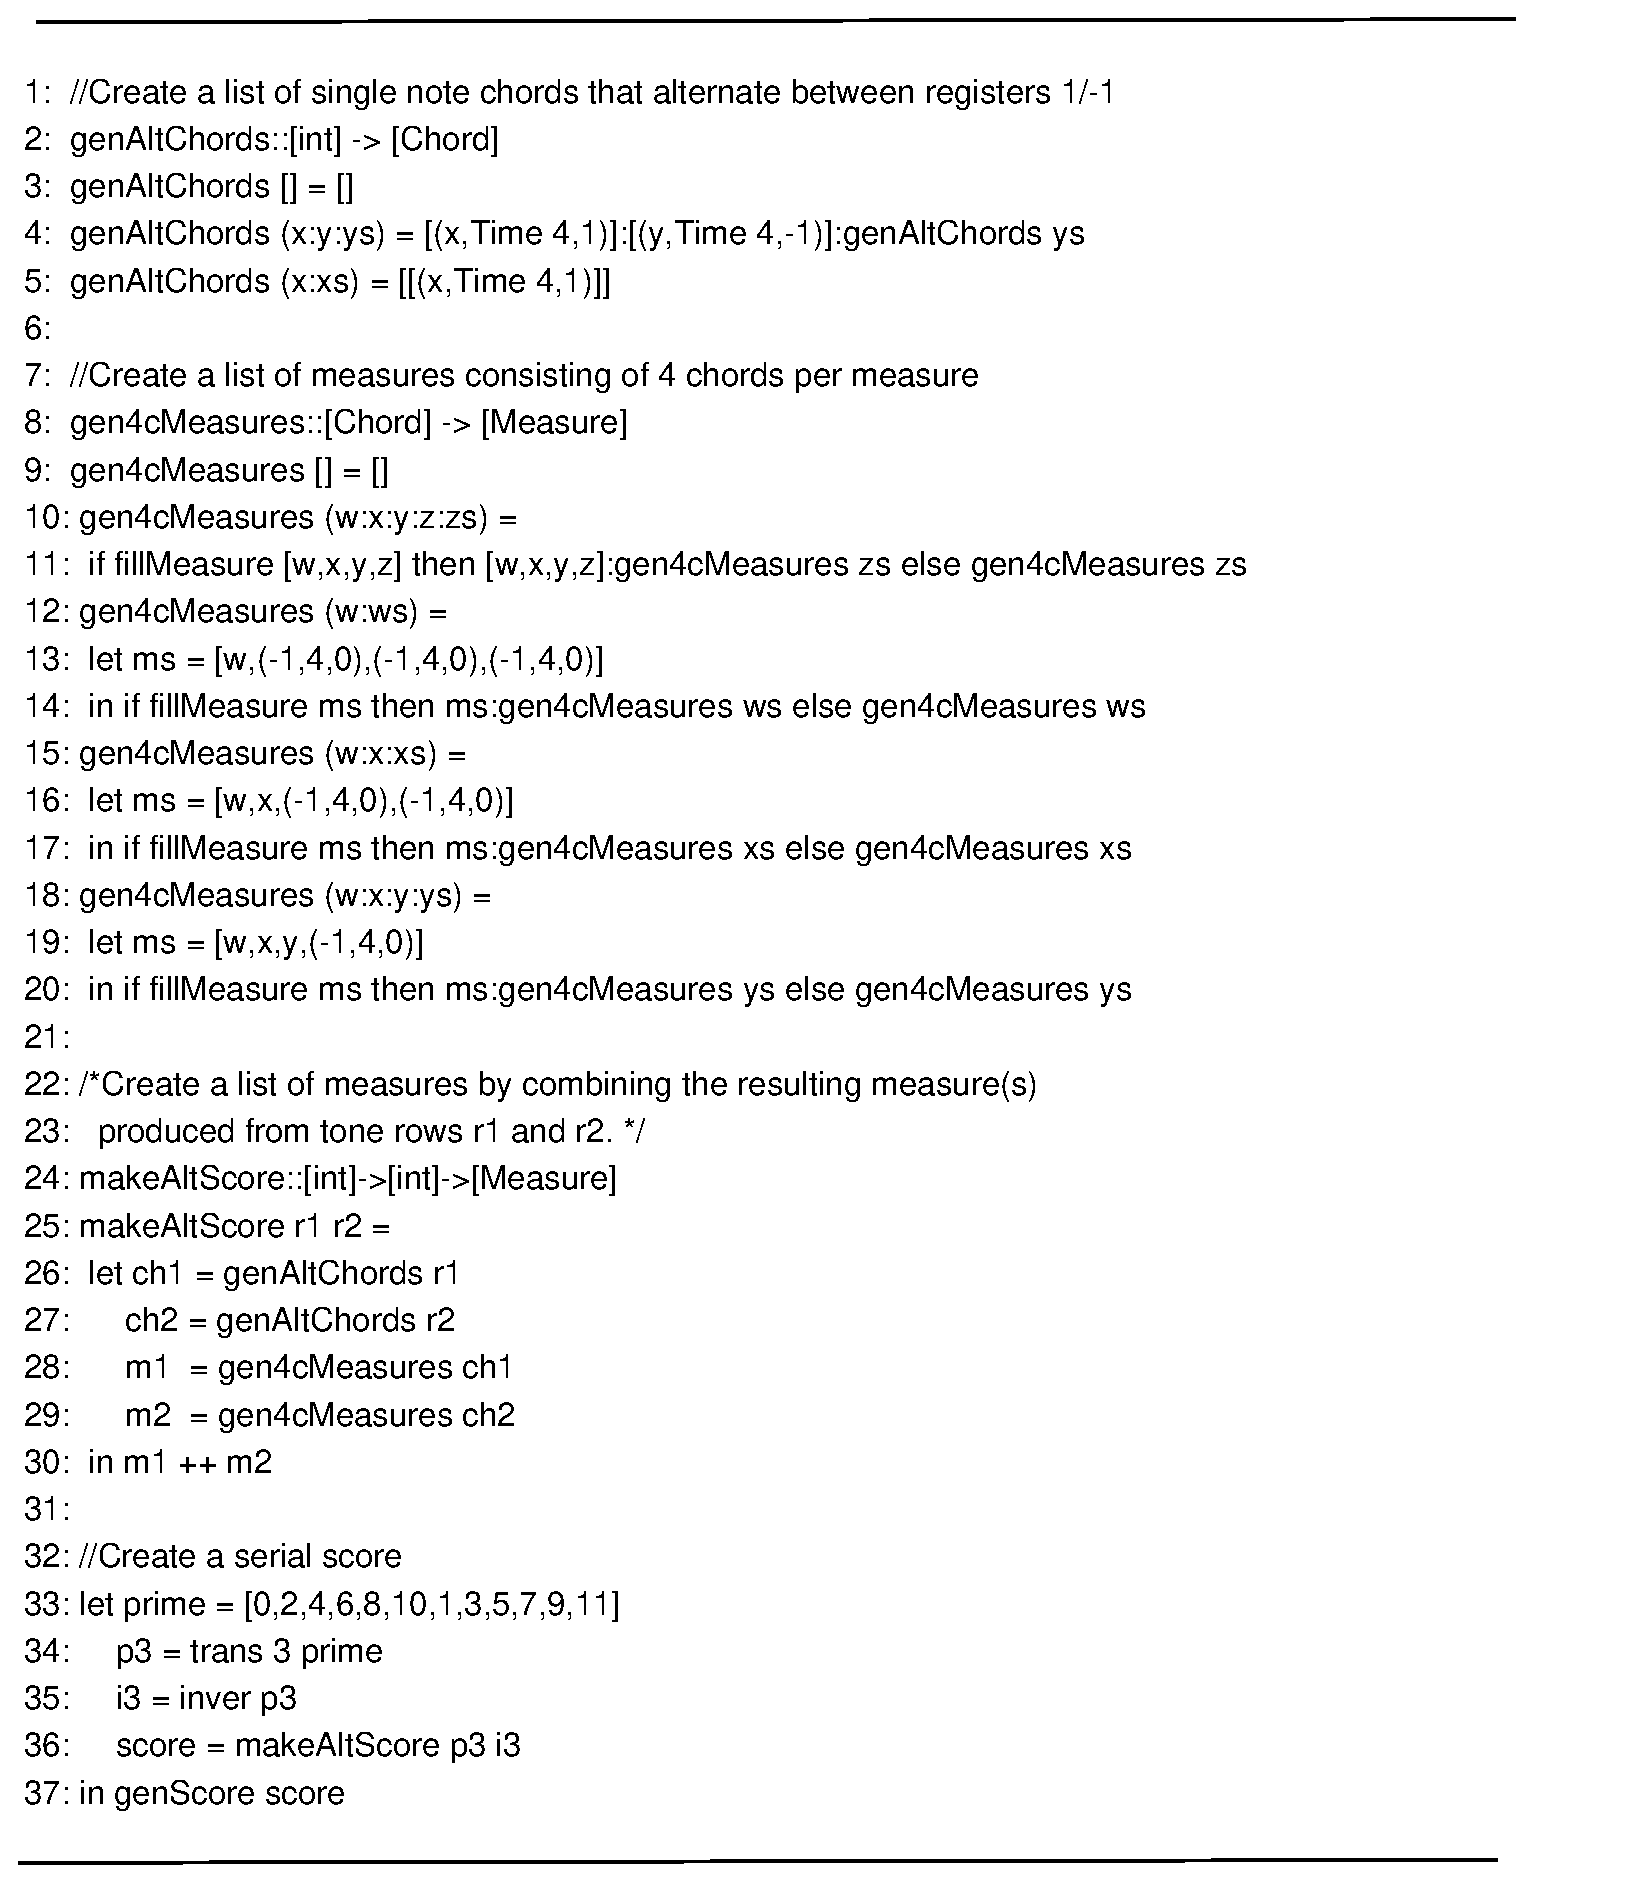
\includegraphics[width=0.75\textwidth]{figures/example1}
        \caption{Example SMURF program.}
        \label{fig:ex1}
\end{figure}

The first step in composing serial music starts with defining the pitch classes for the prime row, which is defined in the example code in line 33.  Using the prime row as a base, the program creates a score using the tone rows generated by transposing the prime row by three semitones (line 34) and inverting the resulting transposed row (line 35). The two tone rows are then passed to the \texttt{makeAltScore} function that creates a list of measures by first invoking \texttt{genAltChords} on the tone rows and then invoking \texttt{gen4cMeasures} on the chords (lines 24-30). The \texttt{genAltChords} function generates a list of single note chords that alternate between the 1 and -1 registers and applies pattern matching and recursion to accomplish this (lines 2-5). The \texttt{gen4cMeasures} function also applies pattern matching and recursion to generate a list of measures using the input chord list. \texttt{gen4cMeasures} uses the library routine \texttt{fillMeasure} to check if a list of chords fills a measure, which is four beats. \texttt{gen4cMeasures} also pads a measure with rest quarter notes if the size of the chord list is less than four in order to fill up the measure.  The score is generated with the \texttt{genScore} keyword using the list of measures (line 37). The SMURF compiler translates the keyword \textbf{genScore} to C+OpenGL code to create a music score sheet.     

% comment out
\iffalse
\small
\begin{verbatim}
1:  //Create a list of single note chords that alternate between registers 1/-1
2:  genAltChords::[int] -> [Chord] 
3:  genAltChords [] = []
4:  genAltChords (x:y:ys) = [(x,Time 4,1)]:[(y,Time 4,-1)]:genAltChords ys
5:  genAltChords (x:xs) = [[(x,Time 4,1)]] 
6: 
7:  //Create a list of measures consisting of 4 chords per measure 
8:  gen4cMeasures::[Chord] -> [Measure] 
9:  gen4cMeasures [] = []
10: gen4cMeasures (w:x:y:z:zs) = 
11:  if fillMeasure [w,x,y,z] then [w,x,y,z]:gen4cMeasures zs else gen4cMeasures zs  
12: gen4cMeasures (w:ws) = 
13:  let ms = [w,(-1,4,0),(-1,4,0),(-1,4,0)]
14:  in if fillMeasure ms then ms:gen4cMeasures ws else gen4cMeasures ws
15: gen4cMeasures (w:x:xs) = 
16:  let ms = [w,x,(-1,4,0),(-1,4,0)]
17:  in if fillMeasure ms then ms:gen4cMeasures xs else gen4cMeasures xs
18: gen4cMeasures (w:x:y:ys) = 
19:  let ms = [w,x,y,(-1,4,0)]
20:  in if fillMeasure ms then ms:gen4cMeasures ys else gen4cMeasures ys
21:
22: /*Create a list of measures by combining the resulting measure(s) 
23:   produced from tone rows r1 and r2. */
24: makeAltScore::[int]->[int]->[Measure]
25: makeAltScore r1 r2 = 
26:  let ch1 = genAltChords r1
27:      ch2 = genAltChords r2
28:      m1  = gen4cMeasures ch1
29:      m2  = gen4cMeasures ch2
30:  in m1 ++ m2 
31:
32: //Create a serial score 
33: let prime = [0,2,4,6,8,10,1,3,5,7,9,11]
34:     p3 = trans 3 prime
35:     i3 = inver p3
36:     score = makeAltScore p3 i3
37: in genScore score
\end{verbatim}
\fi
